\begin{post}
	\postdata{Experience the future (and the past)}{2011}{11}{19}{14}{17}{58}
	\begin{content}
Tuesday was a special day. I got to experience both the future and the past. And no, Dr. Emmet Brown was not involved, and neither was a DeLorean or Marty McFly. But damn, that would be cool if they were. Anyway, on Tuesday, we went to the SK T.um, which is a showroom of SK Telecom, the biggest mobile operator in Korea.

\begin{wrapfigure}{r}{0.3\textwidth}
\vspace{-12pt}\centering\fbox{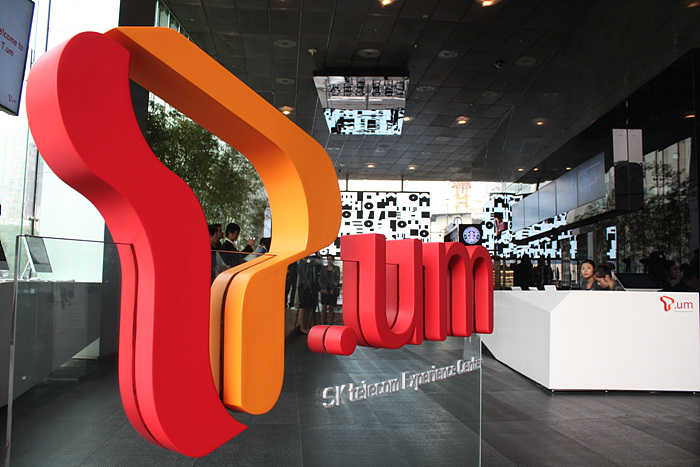
\includegraphics[width=0.3\textwidth]{photos/11/19/IMG_4849.jpg}}
\vspace{-32pt}
\end{wrapfigure}The \textit{``um''} stands for \textit{``Ubiquitous Museum''}, which just seems like a fancy name, because it does not really make sense. However, the whole place is completely awesome, especially for a geek and techie like me.

Firstly, at the beginning of the tour, you receive a Samsung Galaxy S II, which is in T.um terminology called the \textit{T.key}. The phone is equipped with a special \textit{T.um} app and unfortunately it is otherwise locked up (you can't access the underlying Android). After filling in your name, age group, e-mail and telephone, and taking a picture of yourself, you go to a Pond, where your \textit{T.me} (virtual avatar) drops from the ceiling in a form of a water drop \textit{(fancy stuff!)}. The \textit{T.me} then follows you during the whole tour. These things are possible thanks to the integrated ZigBee based short-range communication chip in the phone, which allows it to interact with the objects in the exposition and deliver location based data.

The first part of the tour is called \textbf{``Play Dream''}. It is basically a presentation of \textit{``ubiquitous life service''}, i.e. a service that will be fully integrated into our life.

The first part is dedicated to \textit{Communication and Entertainment}, and it is called the \textit{U.home}. I assume that it stands for ``Ubiquitous Home'', which is, well, something{\ldots}Nah, that \textit{``U''} shit does not make sense. The room is equipped with three beamers that form a huge screen. The screen is controlled by gestures, however, since they use an IR strip and a cam, the recognition is a little slow. Such thing would be much better with a Kinect-like technology. That would make it truly Minority Report-like. Just without the murders and Tom Cruise.

The room also includes a ``multimedia table'', which is something like the Surface table from Microsoft. It is a big screen, that is NFC enabled, so putting the T.key device/mobile phone on the table enables interaction between the table and the phone. That way you can watch movies or pictures from the phone on the table or the big screen without any cables or docks. We made our tour guide play a Girls Generation music video on the huge screen, which made all the guys much happier{\ldots}What I really liked was direct transfer of files between two phones laying on the table. The transfer was however done via 3G/WiFi, as ZigBee is not built for high speed transfer between devices.

The second room was focused on \textit{Gaming (U.entertainment)}. That was a little lame, because using the phone's accelerometer for controlling a game via 3G/WiFi/ZigBee is quite sluggish. We were doing some racing and I finished second, so I am not complaining, but still, it would need improvement for real world deployment. Funny thing was when the guide was reading who is on which position and said ``On the second position is{\ldots}{\ldots}Honza{\ldots}{\ldots}is that your real name?''. Umm, no, madam, I just made it up\ldots

Next part was \textit{``U.driving''}, which included a real car mounted on a hydraulic platform. The car was called Spira, which is a new Korean-made sports car. Morgan and Lauriane were the two ``volunteers'', so they had to go through a simulated ride. The mobile phone acted as a central controller, displaying information about the car (telemetry), serving as a GPS satnav, allowing to pay for the fuel (ehm, electricity) and do other funny things. Frankly, this part was not that impressive, because this is something that will be quite hard to achieve in larger scale, thanks to the fragmentation of in-car systems, but it is a nice concept, that could make driving easier.

While they were still driving, we moved to the next section focused on content creation (\textit{U.media}). In this part our photos from the phone were used to create a 3D advertisement. Since it was just a 2D picture, the photos were simply used as a texture, so you can imagine how it looked. Moreover, the 3D effect was not that good, so I would say this was the weakest part of the exhibition.

\textit{U.fashion}. Girl's heaven, guy's hell. Through a 3D scanner, Karin's body was scanned, analyzed (height and other things) and digitalized. That allowed her to virtually try on various clothes and outfits. I think this might be quite useful, because it saves time and effort. I don't understand why the virtual avatar was standing in a middle of an intersection, though. As usual, the ``app'' allowed you to buy the clothes right after trying them on, without having to leave your home. It would be nice if a 3D printer could print them for you instead:)

%[caption id=``'' align=``aligncenter'' width=``530'' caption=``The 3D full body scanner'']<img class=`` '' title=``The body scanner'' src=``http://sktstory.com/wp-content/uploads/1/499b64f6ede60AZ.jpg'' alt=``'' width=``530'' />[/caption]

Last part of the ``Play Dream'' concept was U.\textit{shopping}. Based on our profile, the system recommended us some goods, which we could directly buy. Every product was associated with some short ``game'', which allowed you to ``try before you buy''. This concept does not seem that impressive, considering the recommendation algorithms used by e-shop or the ``virtual'' shopping mall in the Seoul subway.

Since we were in quite a hurry, we only ran through the second part of the exposition called \textbf{``Play Real''}. While ``the dream'' showcased what will be available in the future, ``the real'' showcased what is already available. There was an augmented reality app for factory controlling, which is supposedly already used, a dock for the mobile that allowed instant switch from the phone to a big TV (erm, HDMI all the way{\ldots}) and a CSR thing, which I did not understand, because I really have no idea what does CSR have in common with visually impaired people.

And that was the end of the tour. We did not get the chance to try out all the gadgets and thingies in the Play Real section, so we just returned our T.keys and went home.

Well, only some of us went home{\ldots}André, Marc and I went for a lunch to Lotteria (Giant Double Burger set FTW!) and then we took a cab to the War Memorial in Yonsan. The WM was the last thing that I really wanted to see among the touristic places in Seoul. And it was also one of the coolest. The memorial, as its name hints, is a museum of all the wars and occupations the Korean peninsula has experienced so far.

\begin{figure}[!h]
\centering
\fbox{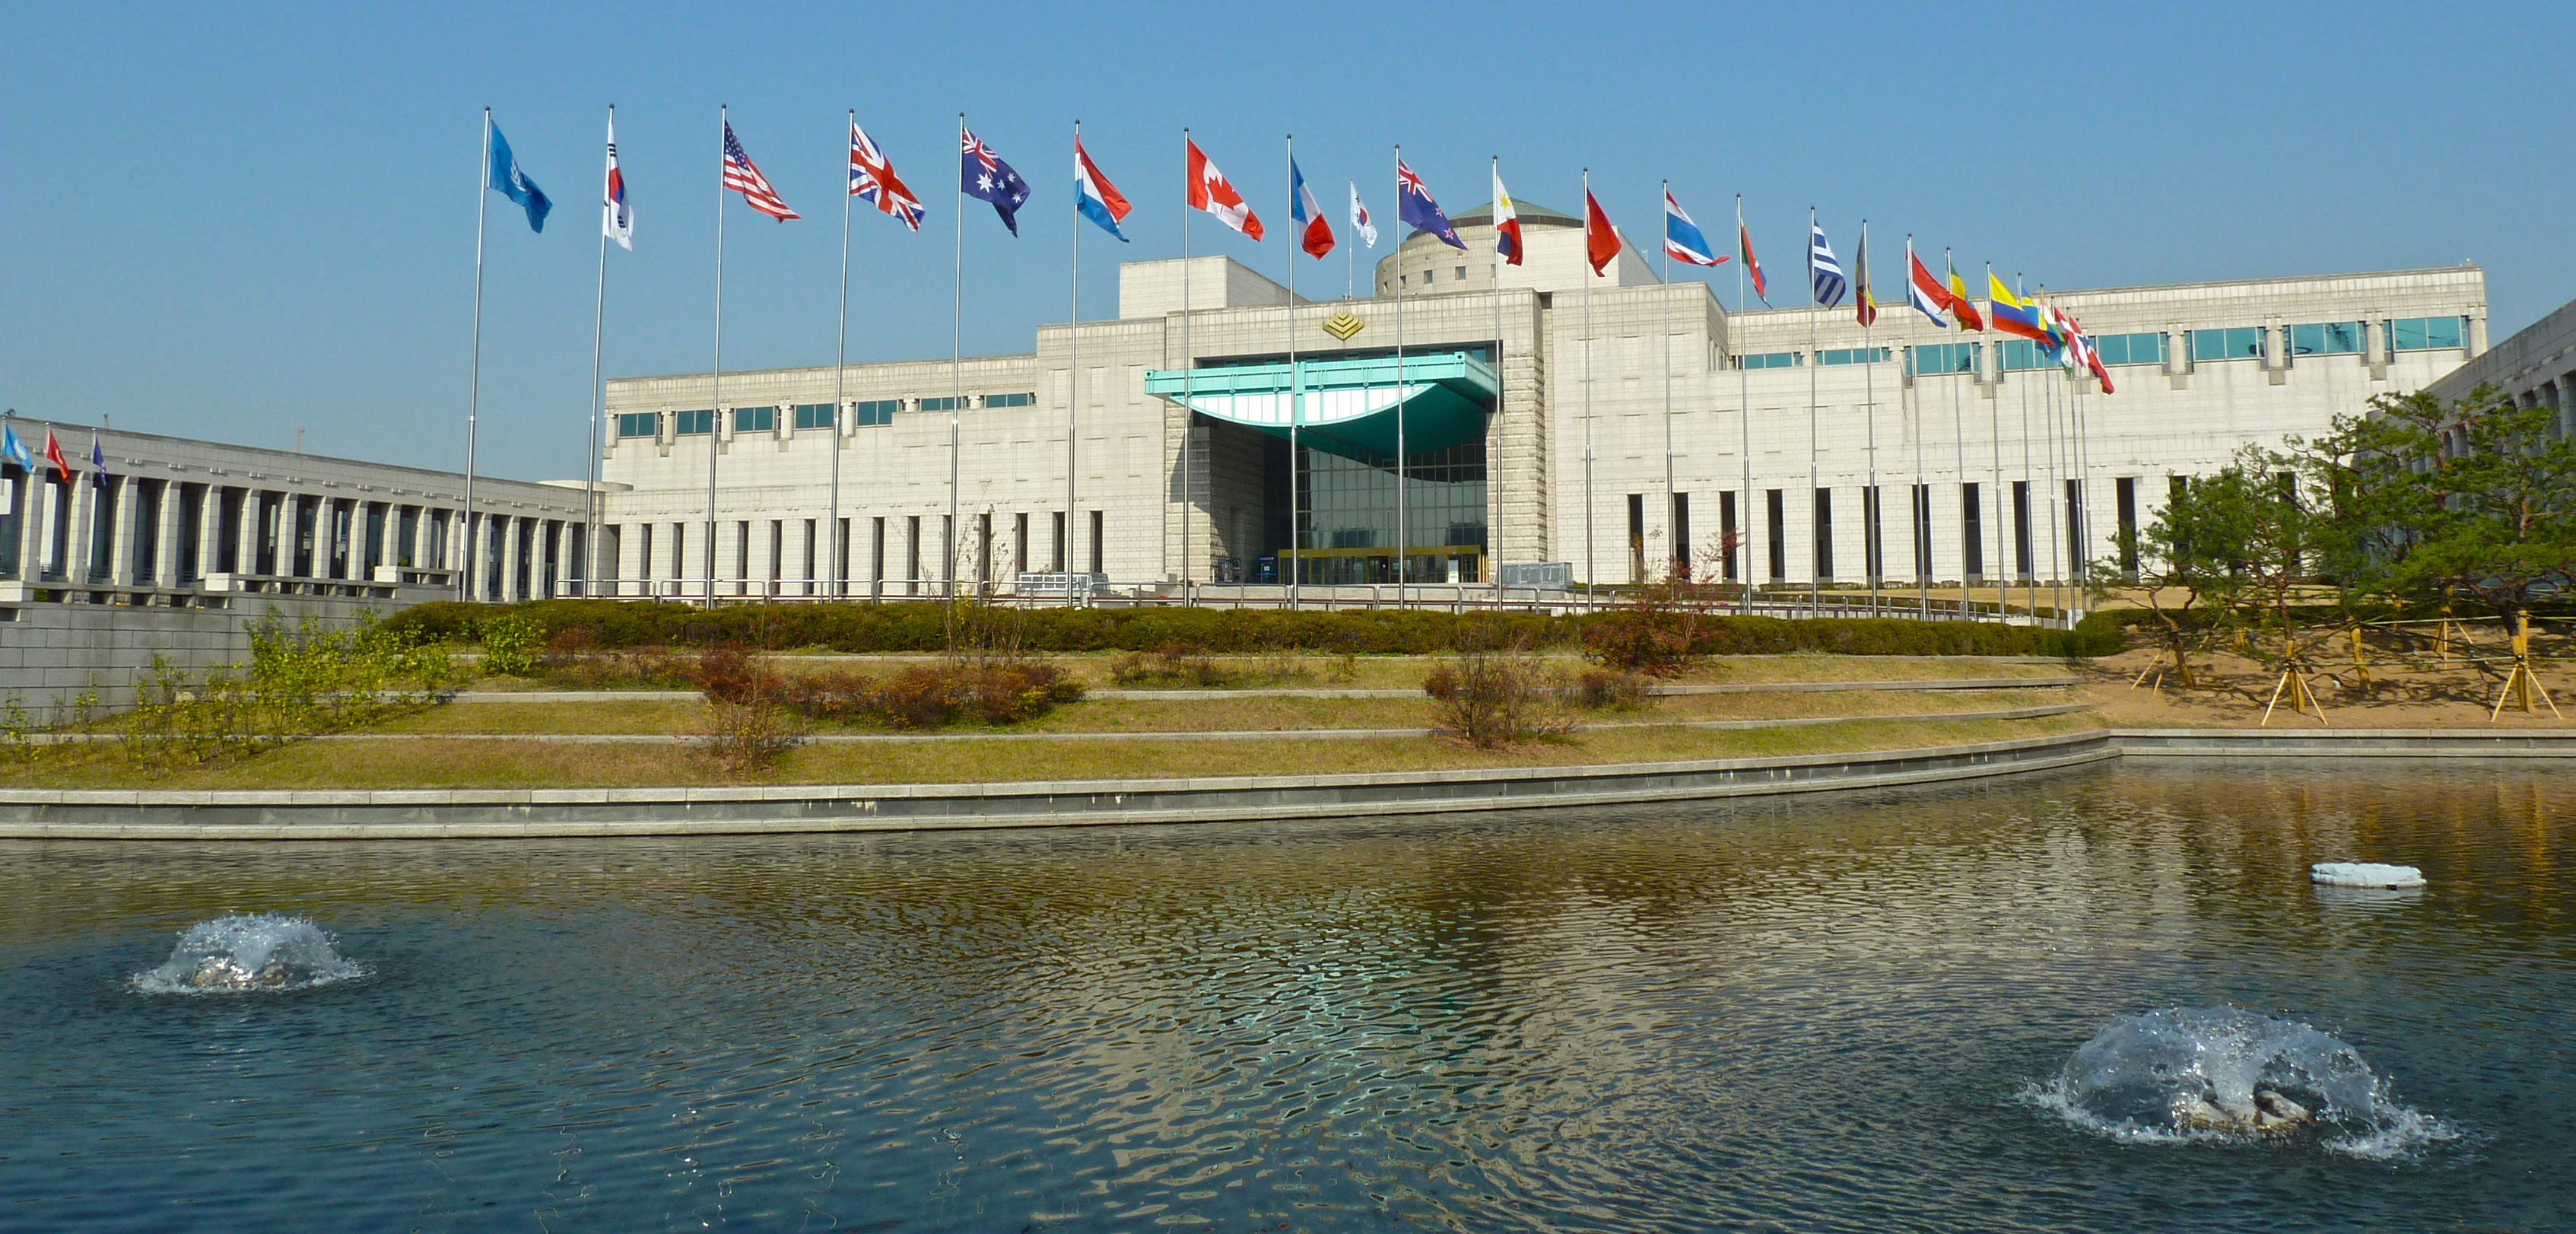
\includegraphics[width=0.6\textwidth]{photos/11/19/p1010471.jpg}}
\caption{The War Memorial}
\end{figure}

The exposition is quite cool, actually. Of course, it is nationalistic and to some extent over-the-top, but that is understandable. This country has been through a lot of wars (almost as much as the Czech Republic), and the scars are still visible. The most notable one is, of course, the DMZ and the separation of the two Koreas. The museum is divided into several rooms, with each one representing different part of Korean military history (Memorial Hall, War History, Korean War, Expeditionary Forces Room, ROK Armed Forces Room, and Large Equipment Room). Each of these rooms displays all the important things, such as uniforms, weapons, paintings of battles etc. Obviously, the biggest part is dedicated to the Korean war, with 3D battle scenes, models, videos etc. There is even a ``Combat Experience Simulator'', which is a simulation of the combat using lights, sounds, smell etc. To absorb all the information in the memorial one would have to spend the whole day there, which we could not since André had a meeting later that afternoon.

\begin{figure}[!h]
\centering
\fbox{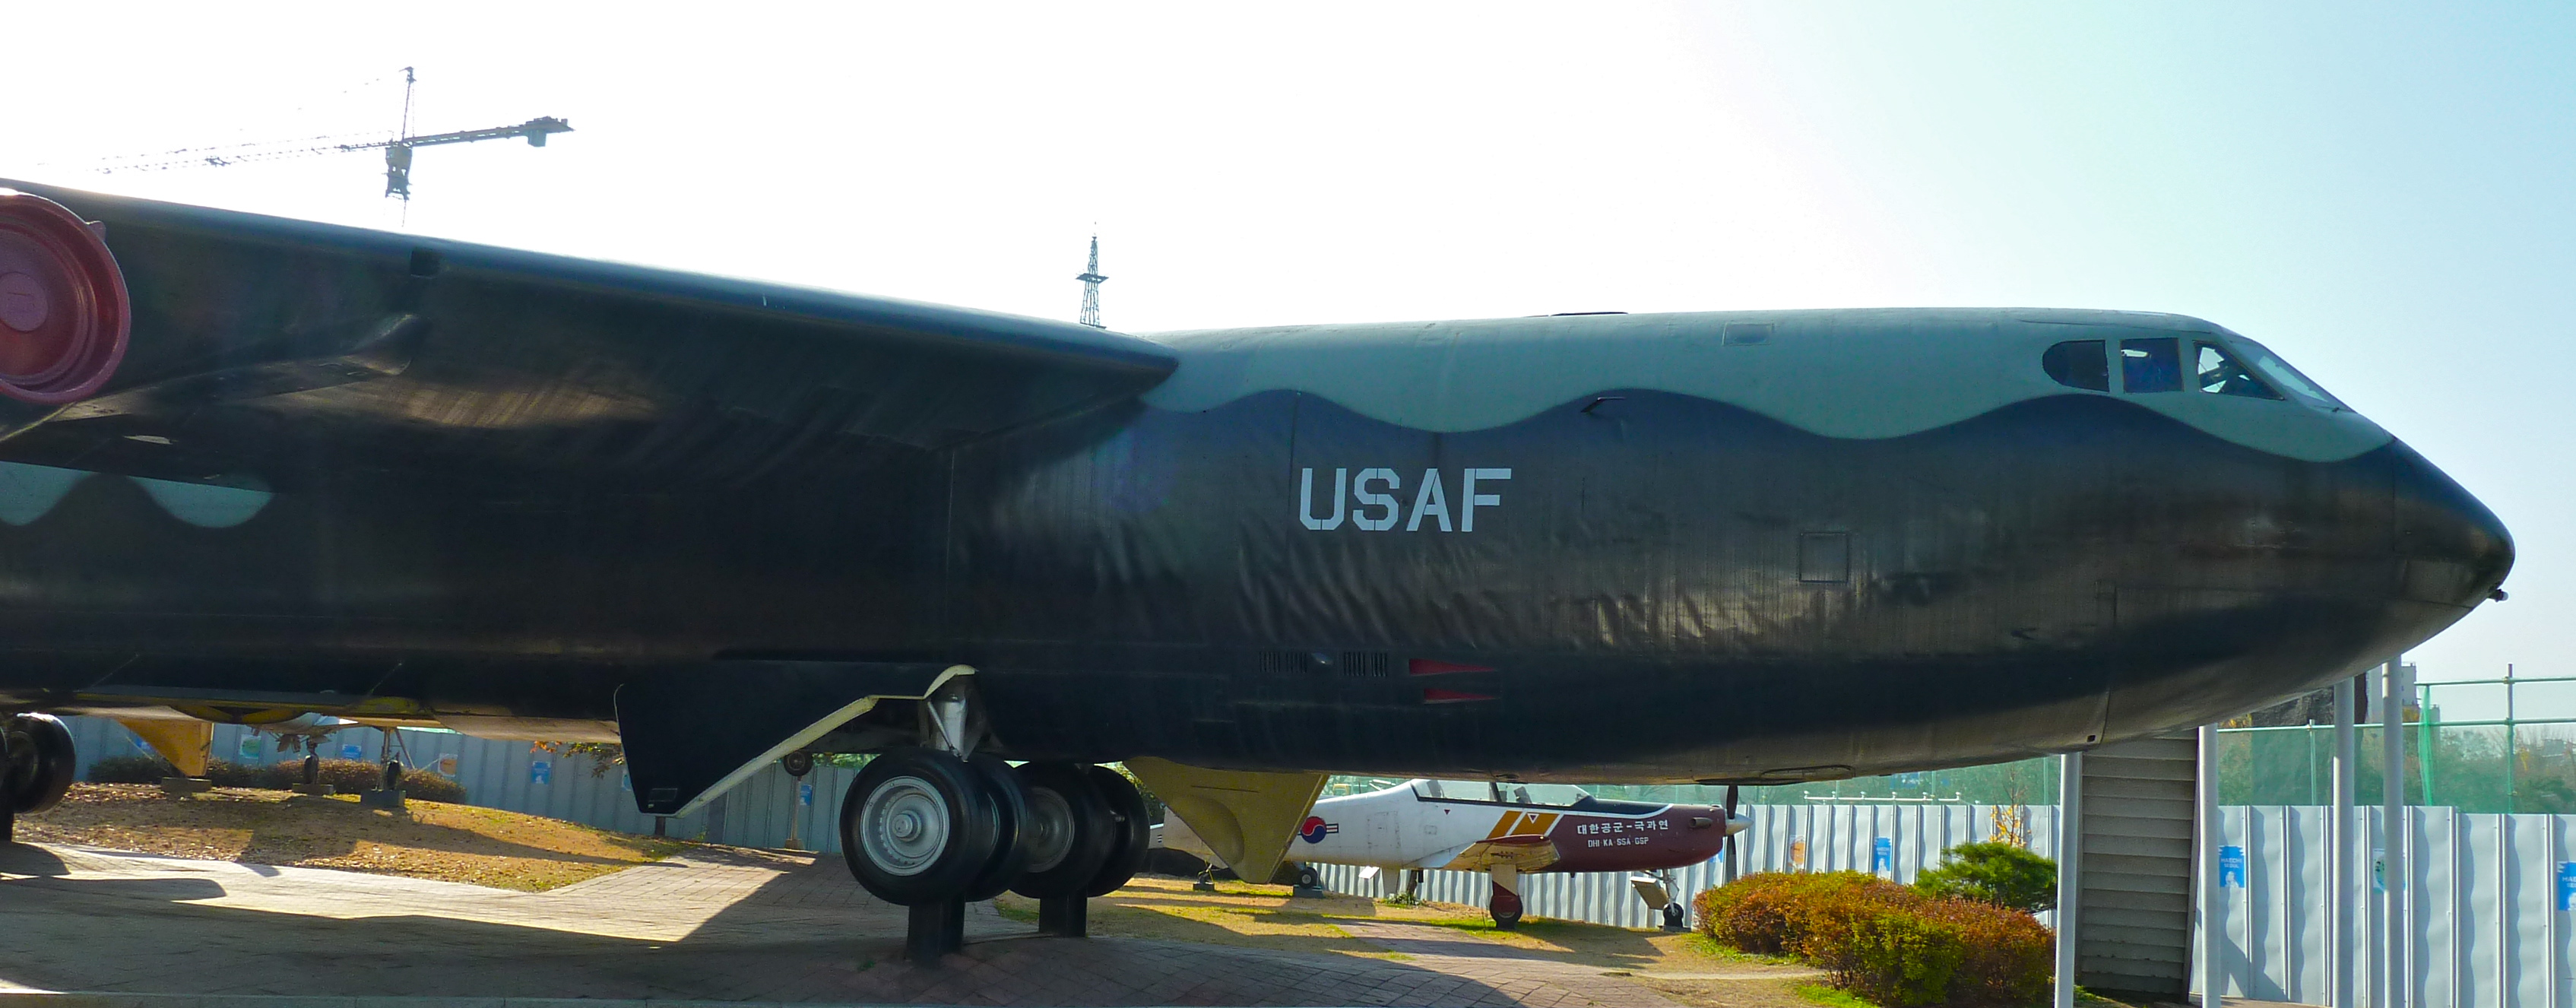
\includegraphics[height=0.25\textwidth]{photos/11/19/p1010478.jpg}}
\caption{A B-52. I would not light this one on fire, though{\ldots}}
\end{figure}

The memorial also has an outside exhibition space, with different pieces of military vehicles and planes. There are both UN/S. Korean and Chinese/USSR/N. Korean machines ranging from AA guns and Howitzers over tanks, armored vehicles and fighter jets to big bombers, such as B-52. There is also a replica of a guard ship that got involved in a naval battle against North Korea, however, I can't remember the details. We were really excited about it --- such place is definitely every guy's dream{\ldots}:)

%[caption id=``attachment_358'' align=``aligncenter'' width=``530'' caption=``A B-52{\ldots}that thing is HUGE!'']<a href=``http://soulexchange.wordpress.com/2011/11/19/experience-the-future-and-the-past/p1010478/'' rel=``attachment wp-att-358''><img class=``size-medium wp-image-358'' title=``A B-52{\ldots}that thing is HUGE!'' src=``http://soulexchange.files.wordpress.com/2011/11/p1010478.jpg?w=530'' alt=``'' width=``530'' height=``207'' /></a>[/caption]

%[caption id=``'' align=``aligncenter'' width=``530'' caption=``Marc and André standing next to the landing gear of a B-52'']<a href=``http://soulexchange.wordpress.com/2011/11/19/experience-the-future-and-the-past/p1010476/'' rel=``attachment wp-att-359''><img title=``B-52 landing gear'' src=``http://soulexchange.files.wordpress.com/2011/11/p1010476.jpg?w=530'' alt=``'' width=``530'' height=``302'' /></a>[/caption]

%[caption id=``attachment_357'' align=``aligncenter'' width=``530'' caption=``&quot;Oh Captain, my Captain{\ldots}&quot; --- André is on a boat!'']<a href=``http://soulexchange.wordpress.com/2011/11/19/experience-the-future-and-the-past/p1010510/'' rel=``attachment wp-att-357''><img class=``size-medium wp-image-357'' title=``Oh Captain, my Captain.'' src=``http://soulexchange.files.wordpress.com/2011/11/p1010510.jpg?w=530'' alt=``Oh Captain, my Captain{\ldots}'' width=``530'' height=``283'' /></a>[/caption] 
	\end{content}
\end{post}
